\documentclass[conference,compsoc]{IEEEtran}
% *** MISC UTILITY PACKAGES ***
%
%\usepackage{ifpdf}
% Heiko Oberdiek's ifpdf.sty is very useful if you need conditional
% compilation based on whether the output is pdf or dvi.
% usage:
% \ifpdf
%   % pdf code
% \else
%   % dvi code
% \fi
% The latest version of ifpdf.sty can be obtained from:
% http://www.ctan.org/pkg/ifpdf
% Also, note that IEEEtran.cls V1.7 and later provides a builtin
% \ifCLASSINFOpdf conditional that works the same way.
% When switching from latex to pdflatex and vice-versa, the compiler may
% have to be run twice to clear warning/error messages.
\usepackage{graphicx}

% *** CITATION PACKAGES ***
%
\ifCLASSOPTIONcompsoc
  % IEEE Computer Society needs nocompress option
  % requires cite.sty v4.0 or later (November 2003)
  \usepackage[nocompress]{cite}
\else
  % normal IEEE
  \usepackage{cite}
\fi
% cite.sty was written by Donald Arseneau
% V1.6 and later of IEEEtran pre-defines the format of the cite.sty package
% \cite{} output to follow that of the IEEE. Loading the cite package will
% result in citation numbers being automatically sorted and properly
% "compressed/ranged". e.g., [1], [9], [2], [7], [5], [6] without using
% cite.sty will become [1], [2], [5]--[7], [9] using cite.sty. cite.sty's
% \cite will automatically add leading space, if needed. Use cite.sty's
% noadjust option (cite.sty V3.8 and later) if you want to turn this off
% such as if a citation ever needs to be enclosed in parenthesis.
% cite.sty is already installed on most LaTeX systems. Be sure and use
% version 5.0 (2009-03-20) and later if using hyperref.sty.
% The latest version can be obtained at:
% http://www.ctan.org/pkg/cite
% The documentation is contained in the cite.sty file itself.
%
% Note that some packages require special options to format as the Computer
% Society requires. In particular, Computer Society  papers do not use
% compressed citation ranges as is done in typical IEEE papers
% (e.g., [1]-[4]). Instead, they list every citation separately in order
% (e.g., [1], [2], [3], [4]). To get the latter we need to load the cite
% package with the nocompress option which is supported by cite.sty v4.0
% and later.





% *** GRAPHICS RELATED PACKAGES ***
%
\ifCLASSINFOpdf
  % \usepackage[pdftex]{graphicx}
  % declare the path(s) where your graphic files are
  % \graphicspath{{../pdf/}{../jpeg/}}
  % and their extensions so you won't have to specify these with
  % every instance of \includegraphics
  % \DeclareGraphicsExtensions{.pdf,.jpeg,.png}
\else
  % or other class option (dvipsone, dvipdf, if not using dvips). graphicx
  % will default to the driver specified in the system graphics.cfg if no
  % driver is specified.
  % \usepackage[dvips]{graphicx}
  % declare the path(s) where your graphic files are
  % \graphicspath{{../eps/}}
  % and their extensions so you won't have to specify these with
  % every instance of \includegraphics
  % \DeclareGraphicsExtensions{.eps}
\fi
% graphicx was written by David Carlisle and Sebastian Rahtz. It is
% required if you want graphics, photos, etc. graphicx.sty is already
% installed on most LaTeX systems. The latest version and documentation
% can be obtained at: 
% http://www.ctan.org/pkg/graphicx
% Another good source of documentation is "Using Imported Graphics in
% LaTeX2e" by Keith Reckdahl which can be found at:
% http://www.ctan.org/pkg/epslatex
%
% latex, and pdflatex in dvi mode, support graphics in encapsulated
% postscript (.eps) format. pdflatex in pdf mode supports graphics
% in .pdf, .jpeg, .png and .mps (metapost) formats. Users should ensure
% that all non-photo figures use a vector format (.eps, .pdf, .mps) and
% not a bitmapped formats (.jpeg, .png). The IEEE frowns on bitmapped formats
% which can result in "jaggedy"/blurry rendering of lines and letters as
% well as large increases in file sizes.
%
% You can find documentation about the pdfTeX application at:
% http://www.tug.org/applications/pdftex





% *** MATH PACKAGES ***
%
\usepackage{amsmath}
% A popular package from the American Mathematical Society that provides
% many useful and powerful commands for dealing with mathematics.
%
% Note that the amsmath package sets \interdisplaylinepenalty to 10000
% thus preventing page breaks from occurring within multiline equations. Use:
%\interdisplaylinepenalty=2500
% after loading amsmath to restore such page breaks as IEEEtran.cls normally
% does. amsmath.sty is already installed on most LaTeX systems. The latest
% version and documentation can be obtained at:
% http://www.ctan.org/pkg/amsmath





% *** SPECIALIZED LIST PACKAGES ***
%
%\usepackage{algorithmic}
% algorithmic.sty was written by Peter Williams and Rogerio Brito.
% This package provides an algorithmic environment fo describing algorithms.
% You can use the algorithmic environment in-text or within a figure
% environment to provide for a floating algorithm. Do NOT use the algorithm
% floating environment provided by algorithm.sty (by the same authors) or
% algorithm2e.sty (by Christophe Fiorio) as the IEEE does not use dedicated
% algorithm float types and packages that provide these will not provide
% correct IEEE style captions. The latest version and documentation of
% algorithmic.sty can be obtained at:
% http://www.ctan.org/pkg/algorithms
% Also of interest may be the (relatively newer and more customizable)
% algorithmicx.sty package by Szasz Janos:
% http://www.ctan.org/pkg/algorithmicx




% *** ALIGNMENT PACKAGES ***
%
%\usepackage{array}
% Frank Mittelbach's and David Carlisle's array.sty patches and improves
% the standard LaTeX2e array and tabular environments to provide better
% appearance and additional user controls. As the default LaTeX2e table
% generation code is lacking to the point of almost being broken with
% respect to the quality of the end results, all users are strongly
% advised to use an enhanced (at the very least that provided by array.sty)
% set of table tools. array.sty is already installed on most systems. The
% latest version and documentation can be obtained at:
% http://www.ctan.org/pkg/array


% IEEEtran contains the IEEEeqnarray family of commands that can be used to
% generate multiline equations as well as matrices, tables, etc., of high
% quality.




% *** SUBFIGURE PACKAGES ***
\ifCLASSOPTIONcompsoc
  \usepackage[caption=false,font=footnotesize,labelfont=sf,textfont=sf]{subfig}
\else
  \usepackage[caption=false,font=footnotesize]{subfig}
\fi
% subfig.sty, written by Steven Douglas Cochran, is the modern replacement
% for subfigure.sty, the latter of which is no longer maintained and is
% incompatible with some LaTeX packages including fixltx2e. However,
% subfig.sty requires and automatically loads Axel Sommerfeldt's caption.sty
% which will override IEEEtran.cls' handling of captions and this will result
% in non-IEEE style figure/table captions. To prevent this problem, be sure
% and invoke subfig.sty's "caption=false" package option (available since
% subfig.sty version 1.3, 2005/06/28) as this is will preserve IEEEtran.cls
% handling of captions.
% Note that the Computer Society format requires a sans serif font rather
% than the serif font used in traditional IEEE formatting and thus the need
% to invoke different subfig.sty package options depending on whether
% compsoc mode has been enabled.
%
% The latest version and documentation of subfig.sty can be obtained at:
% http://www.ctan.org/pkg/subfig




% *** FLOAT PACKAGES ***
%
%\usepackage{fixltx2e}
% fixltx2e, the successor to the earlier fix2col.sty, was written by
% Frank Mittelbach and David Carlisle. This package corrects a few problems
% in the LaTeX2e kernel, the most notable of which is that in current
% LaTeX2e releases, the ordering of single and double column floats is not
% guaranteed to be preserved. Thus, an unpatched LaTeX2e can allow a
% single column figure to be placed prior to an earlier double column
% figure.
% Be aware that LaTeX2e kernels dated 2015 and later have fixltx2e.sty's
% corrections already built into the system in which case a warning will
% be issued if an attempt is made to load fixltx2e.sty as it is no longer
% needed.
% The latest version and documentation can be found at:
% http://www.ctan.org/pkg/fixltx2e


%\usepackage{stfloats}
% stfloats.sty was written by Sigitas Tolusis. This package gives LaTeX2e
% the ability to do double column floats at the bottom of the page as well
% as the top. (e.g., "\begin{figure*}[!b]" is not normally possible in
% LaTeX2e). It also provides a command:
%\fnbelowfloat
% to enable the placement of footnotes below bottom floats (the standard
% LaTeX2e kernel puts them above bottom floats). This is an invasive package
% which rewrites many portions of the LaTeX2e float routines. It may not work
% with other packages that modify the LaTeX2e float routines. The latest
% version and documentation can be obtained at:
% http://www.ctan.org/pkg/stfloats
% Do not use the stfloats baselinefloat ability as the IEEE does not allow
% \baselineskip to stretch. Authors submitting work to the IEEE should note
% that the IEEE rarely uses double column equations and that authors should try
% to avoid such use. Do not be tempted to use the cuted.sty or midfloat.sty
% packages (also by Sigitas Tolusis) as the IEEE does not format its papers in
% such ways.
% Do not attempt to use stfloats with fixltx2e as they are incompatible.
% Instead, use Morten Hogholm'a dblfloatfix which combines the features
% of both fixltx2e and stfloats:
%
% \usepackage{dblfloatfix}
% The latest version can be found at:
% http://www.ctan.org/pkg/dblfloatfix




% *** PDF, URL AND HYPERLINK PACKAGES ***
%
%\usepackage{url}
% url.sty was written by Donald Arseneau. It provides better support for
% handling and breaking URLs. url.sty is already installed on most LaTeX
% systems. The latest version and documentation can be obtained at:
% http://www.ctan.org/pkg/url
% Basically, \url{my_url_here}.




% *** Do not adjust lengths that control margins, column widths, etc. ***
% *** Do not use packages that alter fonts (such as pslatex).         ***
% There should be no need to do such things with IEEEtran.cls V1.6 and later.
% (Unless specifically asked to do so by the journal or conference you plan
% to submit to, of course. )


% correct bad hyphenation here
\hyphenation{}


\begin{document}
%
% paper title
% Titles are generally capitalized except for words such as a, an, and, as,
% at, but, by, for, in, nor, of, on, or, the, to and up, which are usually
% not capitalized unless they are the first or last word of the title.
% Linebreaks \\ can be used within to get better formatting as desired.
% Do not put math or special symbols in the title.
\title{A review of topic model on micro-blogging site using Latent Dirichlet Allocation}


% author names and affiliations
% use a multiple column layout for up to three different
% affiliations
\author{\IEEEauthorblockN{Thuong-Hai Pham}
\IEEEauthorblockA{Faculty of Information and Communication Technology\\
University of Malta\\
Msida MSD 2080, Malta\\
Email: thuong-hai.pham.16@um.edu.mt}
}

% conference papers do not typically use \thanks and this command
% is locked out in conference mode. If really needed, such as for
% the acknowledgment of grants, issue a \IEEEoverridecommandlockouts
% after \documentclass

% for over three affiliations, or if they all won't fit within the width
% of the page (and note that there is less available width in this regard for
% compsoc conferences compared to traditional conferences), use this
% alternative format:
% 
%\author{\IEEEauthorblockN{Michael Shell\IEEEauthorrefmark{1},
%Homer Simpson\IEEEauthorrefmark{2},
%James Kirk\IEEEauthorrefmark{3}, 
%Montgomery Scott\IEEEauthorrefmark{3} and
%Eldon Tyrell\IEEEauthorrefmark{4}}
%\IEEEauthorblockA{\IEEEauthorrefmark{1}School of Electrical and Computer Engineering\\
%Georgia Institute of Technology,
%Atlanta, Georgia 30332--0250\\ Email: see http://www.michaelshell.org/contact.html}
%\IEEEauthorblockA{\IEEEauthorrefmark{2}Twentieth Century Fox, Springfield, USA\\
%Email: homer@thesimpsons.com}
%\IEEEauthorblockA{\IEEEauthorrefmark{3}Starfleet Academy, San Francisco, California 96678-2391\\
%Telephone: (800) 555--1212, Fax: (888) 555--1212}
%\IEEEauthorblockA{\IEEEauthorrefmark{4}Tyrell Inc., 123 Replicant Street, Los Angeles, California 90210--4321}}




% use for special paper notices
%\IEEEspecialpapernotice{(Invited Paper)}




% make the title area
\maketitle

% As a general rule, do not put math, special symbols or citations
% in the abstract
\begin{abstract}
In this paper, the author reviews approaches to apply Latent Dirichlet Allocation (LDA) as a unsupervised topic model for micro-blogging sites. For practical evaluation, Twitter is chosen to do experiment on three approaches: standard LDA, author-topic model and Twitter-LDA. The paper also covers background behind each method and proposes a future works based on these approaches.
\end{abstract}

% no keywords

\section{Introduction}
To deal with the explosion of data these days, especially electronic documents and text generated by world-wide-web users demands techniques that automatically organized large collection of text. One family of those techniques is called "topic model". These techniques discover underlying topic from a given corpus with or without intervention of human, in other word, supervised and unsupervised. One very successful technique and also being considered as state-of-the-art in unsupervised topic model is Latent Dirichlet Allocation (LDA)\cite{Blei2003}.

Applying topic model for micro-blogging site is a very important task to enhance our understanding of the social network. Some applications were proposed by Zhao et al. (2011) \cite{zhao2011comparing} with the work of comparing Twitter and traditional media by LDA, or finding topic-sensitive influencers on Twitter by Weng et al. (2010) \cite{Weng2010}. It is important to be noted that applying LDA on micro-blogging sites is considered a more challenging problem due to the constraint of text length (140 characters in case of Twitter).

\section{Latent Dirichlet Allocation}

\subsection{Bag-of-words assumption}

\subsubsection{Exchangeability}

We say that $(x_1,x_2...)$ is an infinitely exchangeable sequence of random variables if, for any $n$, the joint probability $p(x_1,x_2,...,x_n)$ is invariant to permutation of the indices. That is, for any permutation $\pi$,
\[p(x_1,...,x_n) = p(x_\pi(1),...,x_\pi(n))\]
It is important to emphasize that independent and identically distributed random variables are always infinitely exchangeable. However, infinite exchangeability is a much broader concept than being independent and identically distributed. For example, let $(x_1,x_2,\dots)$ be independent and identically distributed, and let $x_0$ be a non-trivial random variable independent of the rest. Then $(x_0+x_1,x_0+x_2,\dots)$ is infinitely exchangeable but not independent and identically distributed.

\subsubsection{De Finetti theorem, 1935}
A sequence of random variables $(x_1,x_2,...)$ is infinitely exchangeable iff,for all $n$,
\[p(x_1,x_2,...,x_n)=\int\prod_{i=1}^{n}p(x_i|\theta)P(d\theta)\]
for some measure $P$ on $\theta$.
If one assumes the data is infinitely exchangeable, then there must exist an underlying parameter and prior.

\subsection{Latent Dirichlet Allocation}
LDA is a generative probabilistic model of a corpus. The basic idea is that the documents are represented as random mixtures over latent topics, where a topic is characterized by a distribution over words. To implement this idea, LDA assumes each document is a bag-of-words. Hence, it applies infinite exchangeability on the documents and inherits the De Finetti theorem to expect an latent parameter and prior underlying in the corpus. These latent variables are illustrated in the figure \ref{fig:lda_model} below.


\begin{figure}[h]
	\centering
	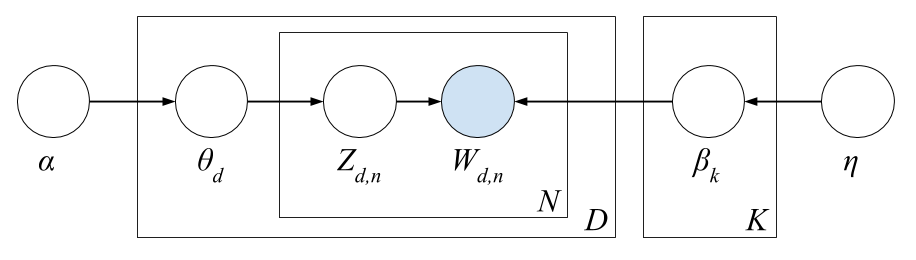
\includegraphics[scale=0.27]{lda_model}
	\caption{LDA graphical model}
	\label{fig:lda_model}
\end{figure}

In figure \ref{fig:lda_model}:
\begin{itemize}
	\item $\alpha$ is Dirichlet distribution parameter, controls the shape and sparsity of $\theta$
	\item $\theta$ are per-document topic proportions.\\
		$\theta$ is a K-dimensional Dirichlet random variable, takes values in the (k-1)-simplex, and has the following probabiltiy density on this simplex:
		\[p(\theta|\alpha)=\frac{\Gamma(\sum_{i=1}^{K}\alpha_i)}{\prod_{i=1}^{K}\Gamma(\alpha_i)}\theta_1^{\alpha_1-1}\dots\theta_K^{\alpha_K-1}\]
		The Dirichlet is conjugate to the multinomial. Given a multinomial observation, the posterior distribution of $\theta$ is a Dirichlet.
	\item $Z_{d,n}$ is per-word topic assignment, in which $D$ and $N$ are number of documents and number of words in a specific document, respectively.
	\item $W_{d,n}$ is observed word.
	\item $\beta$ are topics, which is $V$ dimensional Dirichlet.
	\item $\eta$ is the topic hyper parameter.
\end{itemize}

The blue-shaded node denotes observed variable, the others are hidden or latent variables. Plates denote replicated structures.

 From a collection of documents, LDA infers:
 \begin{itemize}
 	\item Per-word topic assignment $Z_{d,n}$
 	\item Per-document topic proportions $\theta_d$
 	\item Per-corpus topic distributions $\beta_k$
 \end{itemize}

\subsubsection{Generative process}

As mentioned above, LDA is a generative probabilistic model, which generative process is performed as described below:
\begin{enumerate}
	\item Draw $\theta_d \sim Dir(\alpha)$
	\item Draw $\beta_k \sim Dir(\eta)$
	\item For each of the N words in document d $W_{d,n}$:
		\begin{enumerate}
			\item Draw a topic $Z_{d,n} \sim Multinomial(\theta_d)$
			\item Draw a word $W_{d,n}$ from $p(W_{d,n}|Z_{d,n},\beta)$, a multinomial probability conditioned on the topic $Z_{d,n}$
		\end{enumerate}
\end{enumerate}

\subsubsection{Model inference}
However, in the real problem, to acquire underlying latent topics, we have to reverse the generative process by solving an inferential problem. The main goal of this inferential problem is to compute the posterior distribution of the latent variables in figure \ref{fig:lda_model}:
\[p(\theta,Z|W,\alpha,\beta)=\frac{p(\theta,Z,W|\alpha,\beta)}{p(W|\alpha,\beta)}\]

The function $p(\theta,Z|W,\alpha,\beta)$, in practice, is not possible to compute. Due to the conjugacy of Dirichlet distribution, we can marginalize over latent variables to rewrite the posterior $p(W|\alpha,\beta)$. This posterior is still hardly be inferred exactly. Nevertheless, there exist a wide variety of approximate inference algorithms for LDA:
\begin{itemize}
	\item Mean field variational methods \cite{blei2004variational} (Blei et al., 2001)
	\item Expectation propagation \cite{minka2002expectation} (Minka and Lafferty, 2002)
	\item Collapsed Gibbs sampling \cite{griffiths2004finding} (Griffiths and Steyvers, 2004)
	\item Collapsed variational inference \cite{teh2006collapsed} (Teh et al., 2006)
\end{itemize}

After being approximated, beside LDA, the posterior can be used in many other applications such as collaborative filtering, document similarity and information retrieval...

\section{Latent Dirichlet Allocation approaches for Twitter}

One very basic approach is to apply LDA directly to Twitter by treating each tweet as a single document. However, due to the constraint of 140 characters per tweet, a tweet is too short for LDA to figure out the topic proportion.

\subsection{The author-topic model}

To overcome the problem, by assuming that each users on Twitter (Twitterer) only has a fixed interest, aggregating all tweets of a Twitter into a single documents was proposed and gained a better result to direct LDA \cite{Weng2010,hong2010empirical}.

This approach is very efficient on a specific task (ex. topic-sensitive influencers mining \cite{Weng2010}) by not modifying the inference process of original LDA. However, the assumption of the approach is also its disadvantages by the fact that tweets of a Twitterer may generated/tweeted based on a variety of topic that Twitterer pay attention on.

\subsection{Twitter-LDA}

In an attempt to compare Twitter and traditional media, Zhao et al. \cite{zhao2011comparing} proposed Twitter-LDA, a modified version of LDA to work on Twitter's short tweets without assuming that Twitterer has one fixed interest.

\begin{figure}[h]
	\centering
	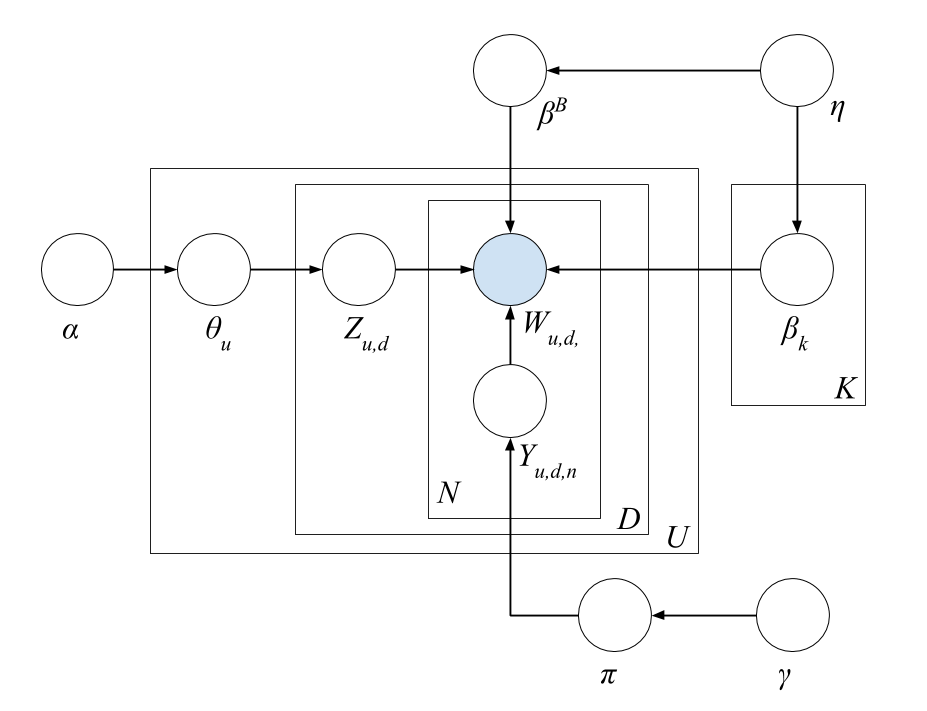
\includegraphics[scale=0.27]{twitter_lda_model}
	\caption{Twitter-LDA graphical model}
	\label{fig:twitter_lda_model}
\end{figure}

In figure \ref{fig:twitter_lda_model}, the author introduced four more variables:
\begin{itemize}
	\item $\beta^B$ denotes the background words distribution
	\item $\pi$ denotes a Bernoulli distribution which simulate the choice of authors between topic-related words and background words.
	\item $\gamma$ is the parameter of distribution $\pi$.
	\item $Y_{u,d,v}$ denotes the selection of background or topic word.
\end{itemize} 
and a slightly modification on $\theta$ that $\theta_u$ denote per-user topic proportions instead of per-document as in the original version. In addition, the D (document) plate is surrounded by a new plate U which stands for each user.

By defining the model as in figure \ref{fig:twitter_lda_model}, the generative process of Twitter-LDA is performed as followed:
\begin{enumerate}
	\item Draw $\beta^B \sim Dir(\eta)$
	\item Draw $\pi \sim Dir(\gamma)$
	\item Draw $\beta_k \sim Dir(\eta)$
	\item For each user,
		\begin{enumerate}
			\item Draw $Z_{u,d} \sim Multi(\theta_u)$
			\item For each word in document d,
				\begin{enumerate}
					\item Draw $Y_{u,d,n} \sim Multi(\pi)$
					\item Draw \[W_{u,d,n} \sim 
					\begin{cases}
						Multi(\theta^B) & \text{if $Y_{u,d,n} = 0$}\\
						Multi(\theta^{Z_{u,d}}) & \text{if $Y_{u,d,n} = 1$}
					\end{cases}\]
				\end{enumerate}
		\end{enumerate}
\end{enumerate}


\section{Evaluation}

\subsection{Evaluation methods}
Wallach et al. \cite{Wallach2009a} summarized a variety of methods to evaluate LDA. As a topic model method, LDA is commonly evaluated by intrinsic and extrinsic evaluation. 

\subsubsection{Intrinsic method}

One very basic intrinsic evaluation method is to view the problem as document modeling \cite{Blei2003}. By stating that, the goal of the model is t achieve high likelihood on a held-out test set, $C'$. In this case, the perplexity measure is used as in normal language modeling problem, in which the lower perplexity, the better performance the model achieves.
\[perp(C')=exp\left\{-\frac{\sum_{d=1}^{D}{log(p(W_d))}}{\sum_{d=1}^{D}N_d}\right\}\]

More advanced, measurement is estimated by the probability of unseen held-out documents given some training documents. This probability can be written as \cite{Wallach2009a}
\[P(C|C')=\int d\theta d\alpha dm P(C|\theta,\alpha m)P(\theta,\alpha m|C').\]
in which, $C, C'$ denote training documents set (corpus) and held-out documents set, respectively. Noted that $m$ is the base measure of Dirichlet distribution, in addition to the concentration parameter $\alpha$.

There is also a variation of this method, document completion, which compare predictive performance by estimating the probability of the second half of each document given the first half. In this point of view, let $c^{(1)}$ be the first half and $c^{(2)}$ be the second half, the goal of our measurement is to compute
\[P(w^{(2)}|w^{(1)},\theta,\alpha m)=\frac{P(w^{(2)}, w^{(1)}|\theta,\alpha m)}{P(w^{(1)}|\theta,\alpha m)}\]

\subsubsection{Extrinsic method}

On the other hand, extrinsic approaches measure LDA performance on some secondary tasks, such as corpus comparison \cite{zhao2011comparing} or topic-sensitive influencers mining \cite{Weng2010}. These approaches are similar to the way language models performance are measured.

\subsection{LDA approaches evaluation result}

As a part of the corpus comparing work \cite{zhao2011comparing}, Zhao et al. also evaluated the performance between original LDA, author-topc model and their proposed Twitter-LDA. Based on preliminary experiments, the authors set number of topic K to 110 for each model, then mixed 330 topics from the three models. The topics were then scored by two human judges. Each assigned a score on each topic, ranging from 1 (meaningful) to 0 (nonsense).

The result showed that Twitter-LDA gained 25.23\% higher in term of average score to author-topic model, and 32.61\% higher then standard LDA. Hence, Twitter-LDA obviously outperformed the two previous methods and were used in their comparison task.

% An example of a floating figure using the graphicx package.
% Note that \label must occur AFTER (or within) \caption.
% For figures, \caption should occur after the \includegraphics.
% Note that IEEEtran v1.7 and later has special internal code that
% is designed to preserve the operation of \label within \caption
% even when the captionsoff option is in effect. However, because
% of issues like this, it may be the safest practice to put all your
% \label just after \caption rather than within \caption{}.
%
% Reminder: the "draftcls" or "draftclsnofoot", not "draft", class
% option should be used if it is desired that the figures are to be
% displayed while in draft mode.
%
%\begin{figure}[!t]
%\centering
%\includegraphics[width=2.5in]{myfigure}
% where an .eps filename suffix will be assumed under latex, 
% and a .pdf suffix will be assumed for pdflatex; or what has been declared
% via \DeclareGraphicsExtensions.
%\caption{Simulation results for the network.}
%\label{fig_sim}
%\end{figure}

% Note that the IEEE typically puts floats only at the top, even when this
% results in a large percentage of a column being occupied by floats.


% An example of a double column floating figure using two subfigures.
% (The subfig.sty package must be loaded for this to work.)
% The subfigure \label commands are set within each subfloat command,
% and the \label for the overall figure must come after \caption.
% \hfil is used as a separator to get equal spacing.
% Watch out that the combined width of all the subfigures on a 
% line do not exceed the text width or a line break will occur.
%
%\begin{figure*}[!t]
%\centering
%\subfloat[Case I]{\includegraphics[width=2.5in]{box}%
%\label{fig_first_case}}
%\hfil
%\subfloat[Case II]{\includegraphics[width=2.5in]{box}%
%\label{fig_second_case}}
%\caption{Simulation results for the network.}
%\label{fig_sim}
%\end{figure*}
%
% Note that often IEEE papers with subfigures do not employ subfigure
% captions (using the optional argument to \subfloat[]), but instead will
% reference/describe all of them (a), (b), etc., within the main caption.
% Be aware that for subfig.sty to generate the (a), (b), etc., subfigure
% labels, the optional argument to \subfloat must be present. If a
% subcaption is not desired, just leave its contents blank,
% e.g., \subfloat[].


% An example of a floating table. Note that, for IEEE style tables, the
% \caption command should come BEFORE the table and, given that table
% captions serve much like titles, are usually capitalized except for words
% such as a, an, and, as, at, but, by, for, in, nor, of, on, or, the, to
% and up, which are usually not capitalized unless they are the first or
% last word of the caption. Table text will default to \footnotesize as
% the IEEE normally uses this smaller font for tables.
% The \label must come after \caption as always.
%
%\begin{table}[!t]
%% increase table row spacing, adjust to taste
%\renewcommand{\arraystretch}{1.3}
% if using array.sty, it might be a good idea to tweak the value of
% \extrarowheight as needed to properly center the text within the cells
%\caption{An Example of a Table}
%\label{table_example}
%\centering
%% Some packages, such as MDW tools, offer better commands for making tables
%% than the plain LaTeX2e tabular which is used here.
%\begin{tabular}{|c||c|}
%\hline
%One & Two\\
%\hline
%Three & Four\\
%\hline
%\end{tabular}
%\end{table}


% Note that the IEEE does not put floats in the very first column
% - or typically anywhere on the first page for that matter. Also,
% in-text middle ("here") positioning is typically not used, but it
% is allowed and encouraged for Computer Society conferences (but
% not Computer Society journals). Most IEEE journals/conferences use
% top floats exclusively. 
% Note that, LaTeX2e, unlike IEEE journals/conferences, places
% footnotes above bottom floats. This can be corrected via the
% \fnbelowfloat command of the stfloats package.

\section{Conclusion}
The two proposed methods of author-topic model and Twitter-LDA have overcome the problem of short tweets in the micro-blogging site Twitter. More than that, Twitter-LDA has showed to outperform the other two in experiment.

However, Twitter-LDA has to change the original LDA process and inference approximation algorithm to implement its idea. This approach is hard to be re-implemented in industrial by using existed library for other problems. We argue that aggregating into a single document may fail to model topic(s) of influencers who have more than one field of interest and/or change their interest from time to time. Hence, the two following scenarios should be the future work to solve the problem without modifying the original LDA process:
\begin{enumerate}
	\item Applying LDA on a single user, each tweet as a document, then group these documents based on their LDA-topics.
	\item Grouping tweets based on their tweeted/retweeted timestamp.
\end{enumerate}
After processing the corpus by one of these above mentioned methods, we treat the grouped tweets as a single document to apply LDA.


% trigger a \newpage just before the given reference
% number - used to balance the columns on the last page
% adjust value as needed - may need to be readjusted if
% the document is modified later
%\IEEEtriggeratref{8}
% The "triggered" command can be changed if desired:
%\IEEEtriggercmd{\enlargethispage{-5in}}

% references section

% can use a bibliography generated by BibTeX as a .bbl file
% BibTeX documentation can be easily obtained at:
% http://mirror.ctan.org/biblio/bibtex/contrib/doc/
% The IEEEtran BibTeX style support page is at:
% http://www.michaelshell.org/tex/ieeetran/bibtex/
%\bibliographystyle{IEEEtran}
% argument is your BibTeX string definitions and bibliography database(s)
%\bibliography{IEEEabrv,../bib/paper}
%
% <OR> manually copy in the resultant .bbl file
% set second argument of \begin to the number of references
% (used to reserve space for the reference number labels box)
\bibliographystyle{IEEEtran}
\bibliography{summarize}


\end{document}
